This is the description and methodology.

\subsection{Configuration of the STK1000}

\subsubsection{Jumpers}

The STK1000 has 10 jumpers that can be set to configure the board.
For this assignment the jumpers were set as specified on page 37 in \cite{lab-compendium}.


\subsubsection{GPIO connections}

The STK1000 provides a general purpose input/output interface (\texttt{GPIO}) with 32 signal lines.
16 of the 32 available lines were connected to on-board I/O devices on the STK1000 in this assignment.
The I/O devices in use were 8 on-board LEDs, used as a rudimentary paddle display, and 8 on-board switches, used as player controls.

The buttons were connected to \texttt{GPIO0-GPIO7} (\texttt{J1} on the STK1000) using a flat cable as in figure \ref{flat-cable-image}. This maps the buttons to ports \texttt{0-7} of \texttt{PIOB}.
The choice of low port numbers \texttt{0-7} is convenient for coding, and the choice of \texttt{PIOB} as opposed to \texttt{PIOC} is purely mnemonic ('B' for buttons).

The LEDs were connected to \texttt{GPIO16-GPIO23} (\texttt{J3} on the STK1000) using a flat cable as in figure \ref{flat-cable-image}. This maps the LEDs to ports \texttt{0-7} of \texttt{PIOC}.
Having the same port numbers for the buttons and the LEDs is a nice convenience for cleaner and more efficient code, as translation from button ports to LED ports is not necessary.

\begin{figure}
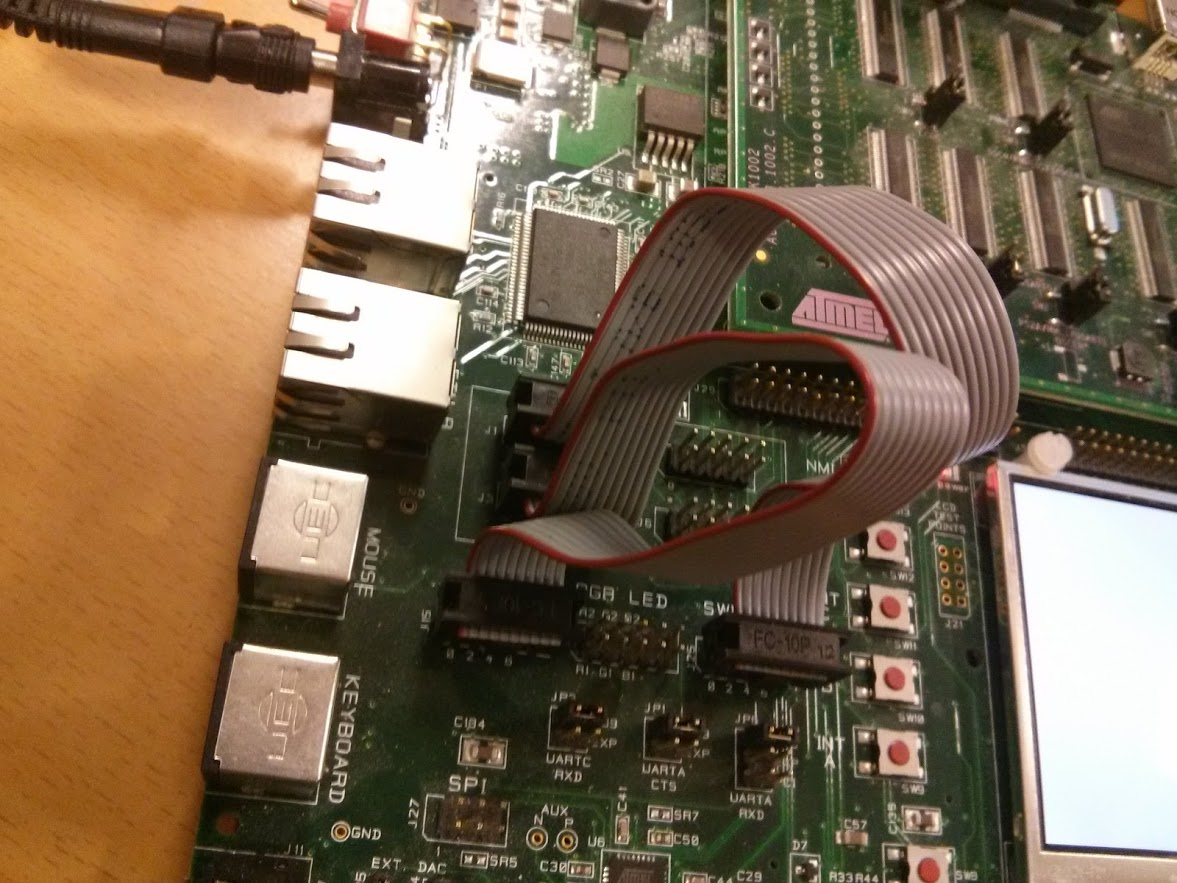
\includegraphics[width = \textwidth]{description-and-methodology/flat-cable-image.jpg}
\caption{Flat cables connecting GPIO with switches and LEDs. Note the orientation of the flat cables.}
\label{flat-cable-image}
\end{figure}


\subsection{Programming environment}

\subsubsection{JTAGICE}

The AP7000 sisterboard on the STK1000 provides a JTAG interface, which is used for programming and debugging of the board.
The development PC was connected to the JTAG interface of the STK1000 using an Atmel JTAGICE mk II (firmware 7.29).
The JTAGICE does not require external power as long as it is connected to the PC over USB.


\subsubsection{GNU Debugger}

\subsubsection{Make, other tools etc}

\subsection{Development of the program}

\subsubsection{Setting up the LED diodes}

\subsubsection{Setting up the buttons}

\subsubsection{Interrupt Routine}

\subsubsection{Refactoring and Modularization}

\subsubsection{Register Overview}

<description of which registers do what>

\subsubsection{Program flow}

<diagrams, descriptions>

yuml.me-source for diagrams

Main program flow:
(start)->(Init)->(Main loop)->(Main loop)


Init:
(start)->(Load pointers)->(Set up start values in registers)->(Enable I/O with interrupts)->(end)

Main loop:
(start)->(Set leds)->(Sleep)[interrupt]-><interrupt routine>->[Was SW0 pressed][Yes]->(Move paddle right)->(end),[Was SW0 pressed][No]->(Move paddle left)->(end)


Set leds:
(start)->(Turn off all LEDs)->(Turn on the paddle LED)->(end)

Button interrupt routine:
(start)->(Read button states)->(Software debounce)->(Notify that the interrupt has been handled)->(end)

Debounce:
(start)->(Set register to a high constant)->(Is value in register equal to 0)[Yes]->(end),(Is value in register equal to 0)[No]->(Decrease value in register by 1)->(Is value in register equal to 0)

Read buttons:
(start)->(Read button status)->(Mask away buttons that were pressed in previous interrupt)->(end)

Move paddle right:
(start)->(Is paddle at far-right end of the board)[Yes]->(Move paddle to far-left)->(end),(Is paddle at far-right end of the board)[No]->(Move paddle one step to the left)->(end)

Move paddle left (analogous to move paddle right, but included for completeness):
(start)->(Is paddle at far-left end of the board)[Yes]->(Move paddle to far-right)->(end),(Is paddle at far-left end of the board)[No]->(Move paddle one step to the right)->(end)



